\chapter{Architettura del Software e Logica di Rendering}

Il presente capitolo illustra la struttura interna del sistema di generazione delle immagini, descrivendo come i moduli che lo compongono cooperino per trasformare un segnale ECG digitale in un'immagine sintetica pronta per l'addestramento di modelli di Deep Learning. Il sistema è stato sviluppato a partire dalla repository pubblica \textit{ECG-Image-Kit}~\cite{ecgimagekitpaper}, sulla quale sono state apportate significative estensioni e modifiche al fine di aumentarne la flessibilità, le prestazioni e la varietà dell'output prodotto.

\section{Struttura Modulare del Progetto}

Il software è organizzato secondo una architettura a strati ben separati, in cui ogni modulo è responsabile di una fase specifica della pipeline. I due script principali (\texttt{gen\_ecg\_images\allowbreak{}\_from\_\allowbreak{}data\_batch.py} e \texttt{gen\_ecg\_image\allowbreak{}\_from\_\allowbreak{}data.py}) costituiscono i punti di ingresso della pipeline, rispettivamente per l'elaborazione in modalità batch e per la generazione da un singolo file. Il nucleo del rendering è contenuto in \texttt{ecg\_plot.py}, mentre la logica di estrazione e segmentazione del segnale risiede in \texttt{extract\_leads.py}. I sottomoduli \texttt{HandwrittenText}, \texttt{CreasesWrinkles} e \texttt{ImageAugmentation} sono responsabili delle fasi di applicazione degli artefatti all'immagine, descritte in dettaglio nel Capitolo~3.

\begin{figure}[H]
\centering
\begin{dirtree}{%
.1 ecg-image-generator/.
.2 gen\_ecg\_images\_from\_data\_batch.py.
.2 gen\_ecg\_image\_from\_data.py.
.2 extract\_leads.py.
.2 ecg\_plot.py.
.2 helper\_functions.py.
.2 config.yaml.
.2 HandwrittenText/.
.3 generate.py.
.3 pretrained/.
.2 CreasesWrinkles/.
.3 creases.py.
.3 wrinkles-dataset/.
.2 ImageAugmentation/.
.3 augment.py.
.2 Fonts/.
.2 TemplateFiles/.
.2 SampleData/.
}
\caption{Struttura delle directory del modulo \textit{ecg-image-generator}.}
\label{fig:dirtree}
\end{dirtree}
\end{figure}

\section{Formati dei Dati in Ingresso}

Il sistema supporta due formati di input selezionabili tramite il parametro \texttt{--dataset\_format}: il formato \textit{WFDB} usato dal dataset PTB-XL e il formato HDF5 usato dal dataset CODE-15\%.

\subsection{Formato WFDB (PTB-XL)}

Il formato \textit{WFDB} (WaveForm DataBase), definito da PhysioNet~\cite{PhysioNet-ptb-xl-1.0.3}, costituisce lo standard \textit{de facto} per i dataset di segnali biomedici pubblicamente disponibili. Ogni registrazione è composta da due file distinti, ai quali si aggiunge un file CSV di metadati condiviso tra tutti i record del dataset:

\begin{itemize}
    \item \textbf{File Header (.hea):} Metadati tecnici, in formato testuale (frequenza campionamento, gain, baseline, nomi derivazioni).
    \item \textbf{File Dati (.dat):} Segnale binario grezzo (16-bit) per le 12 derivazioni.
    \item \textbf{File Metadati (.csv):} Dati paziente (id, età, sesso, diagnosi) e indicatori di qualità (rumore, drift, artefatti) per il controllo del rendering.
\end{itemize}

Il modulo \texttt{helper\_functions.py} espone le funzioni di basso livello per il parsing di questi file. La funzione \texttt{load\_header()} legge il file \texttt{.hea} come stringa, da cui vengono estratti la frequenza di campionamento tramite \texttt{get\_frequency()}, i nomi delle derivazioni tramite \texttt{get\_leads()} e i guadagni ADC tramite \texttt{get\_adc\_gains()}. Il segnale grezzo viene poi caricato da \texttt{load\_recording()}, che utilizza la libreria \texttt{wfdb} per i file \texttt{.dat} e \texttt{scipy.io} per i file \texttt{.mat}, restituendo in entrambi i casi una matrice NumPy di forma \texttt{(campioni, derivazioni)}.

Un passaggio critico è la normalizzazione dei nomi delle derivazioni, gestita da \texttt{standardize\_leads()}: la funzione uniforma le convenzioni di notazione, convertendo in maiuscolo le derivazioni standard (es. \texttt{i} $\rightarrow$ \texttt{I}) e applicando la notazione camelCase per le derivazioni aumentate (\texttt{avr} $\rightarrow$ \texttt{aVR}, \texttt{avl} $\rightarrow$ \texttt{aVL}, \texttt{avf} $\rightarrow$ \texttt{aVF}).

\subsection{Formato HDF5 (CODE-15\%)}

Il supporto al dataset CODE-15\%~\cite{ribeiro_2021_4916206} è stato introdotto come contributo originale in questo lavoro. CODE-15\% è un dataset pubblico di ECG a 12 derivazioni raccolto in Brasile, con frequenza di campionamento di 400 Hz; i segnali sono distribuiti in file HDF5 (\texttt{.hdf5}), ciascuno contenente un tensore di forma \texttt{(N, 4096, 12)}, dove 4096 è la lunghezza fissa del buffer per esame, accompagnato da un vettore di identificatori \texttt{exam\_id}. I metadati clinici (età, sesso, diagnosi) sono forniti separatamente nel file \texttt{exams.csv}, passato al sistema tramite il parametro \texttt{--csv\_file}.

La scansione dei file HDF5 è gestita dalla funzione \texttt{find\_code15\_records()}: essa percorre la directory (o il singolo file) specificata da \texttt{-i}, legge i vettori \texttt{exam\_id} da ogni file HDF5 tramite la libreria \texttt{h5py}, e restituisce la lista di tutti i record come dizionari contenenti il percorso HDF5, l'indice dell'esame nel tensore e l'identificatore univoco. Per robustezza, la funzione gestisce automaticamente le due varianti di denominazione dei dataset HDF5 presenti nelle diverse versioni del dataset (\texttt{tracings}/\texttt{exam\_id} oppure \texttt{signal}/\texttt{id\_exam}).

\section{Pipeline di Elaborazione Batch}\label{sec:batch}

L'elaborazione di un intero dataset è gestita da \texttt{gen\_ecg\_images\_from\_data\_batch.py}. Il flusso è il seguente:

\begin{enumerate}
    \item \textbf{Scansione della directory di input:} il comportamento dipende dal parametro \texttt{--dataset\_format}. In modalità \texttt{ptbxl} (default) la funzione \texttt{find\_records()} percorre ricorsivamente la directory cercando file \texttt{.dat} o \texttt{.mat}, accoppiando ciascun file dati con il corrispondente header \texttt{.hea}; la struttura di sottodirectory viene replicata nella cartella di output. In modalità \texttt{code15} la funzione \texttt{find\_code15\_records()} scansiona i file HDF5 presenti nella directory (o il singolo file indicato) e restituisce la lista di tutti gli esami, identificati da percorso HDF5 e indice nel tensore.
    \item \textbf{Preparazione dei task:} per ogni record viene creata una copia degli argomenti di configurazione, con i percorsi di input e output specifici. Il layout di colonne viene determinato automaticamente in base al parametro \texttt{--layout} scelto.
    \item \textbf{Esecuzione parallela:} i task vengono distribuiti su un pool di processi tramite \texttt{ProcessPoolExecutor}, che sfrutta la parallelizzazione a livello di processo per aggirare il Global Interpreter Lock (GIL) di Python. Una soluzione basata su \texttt{ThreadPoolExecutor} è stata valutata ma scartata: il GIL impedisce l'esecuzione simultanea di bytecode Python su thread distinti, rendendo il parallelismo a thread inefficace per workload CPU-bound come quello in esame. L'utilizzo di processi separati, ciascuno con il proprio interprete e heap, consente invece la vera esecuzione concorrente su più core fisici. L'unica risorsa logicamente condivisa tra i processi è il file CSV dei metadati. Poiché l'accesso avviene esclusivamente in modalità \textit{read-only}, il sistema operativo consente aperture concorrenti del file senza necessità di meccanismi di sincronizzazione espliciti o serializzazione artificiale, garantendo così la massima scalabilità durante la generazione parallela del dataset. Il meccanismo, introdotto come contributo originale al progetto, ha ridotto sensibilmente i tempi di generazione su dataset di grandi dimensioni come PTB-XL, che conta oltre 21\,000 registrazioni. Il carico di lavoro si presta in modo naturale alla parallelizzazione: ogni record ECG è un'unità di elaborazione completamente indipendente dalle altre, priva di stato condiviso tra task distinti. La generazione di ciascuna immagine coinvolge operazioni computazionalmente intensive, rendering vettoriale, applicazione di artefatti grafici e augmentazione, che non richiedono sincronizzazione né comunicazione tra processi. Questo pattern \textit{embarrassingly parallel} permette di saturare efficacemente tutti i core disponibili, con un overhead di coordinamento trascurabile rispetto al costo di ogni singolo task.
    \item \textbf{Monitoraggio e statistiche:} una barra di avanzamento \texttt{tqdm} mostra in tempo reale lo stato della generazione. Il processo può essere interrotto dall'utente in qualsiasi momento tramite segnale di interruzione ({\ttfamily Ctrl+C}): in tal caso, i task già completati vengono preservati e il sistema stampa comunque le statistiche parziali relative alle immagini generate fino a quel momento, numero di immagini prodotte, tempo trascorso e immagini per secondo.
\end{enumerate}

Ogni task viene eseguito dalla funzione \texttt{run\_single\_file()} definita in \texttt{gen\_ecg\_image\_from\_data.py}, che costituisce il nucleo dell'intera pipeline di generazione per un singolo record.

\section{Segmentazione del Segnale e Gestione dei Layout}

La funzione \texttt{get\_paper\_ecg()} in \texttt{extract\_leads.py} gestisce la conversione del segnale in frame pronti per il rendering. Il segnale ECG, tipicamente della durata di 10 secondi, viene suddiviso in finestre temporali la cui estensione dipende dal layout scelto.

\subsection{Layout Supportati}

Il sistema supporta quattro configurazioni di stampa, che replicano i formati utilizzati nella pratica clinica:

\begin{itemize}
    \item \textbf{$12\times1$:} tutte e 12 le derivazioni disposte in una singola colonna. Ogni derivazione mostra 10 secondi di segnale.
    \item \textbf{$6\times2$:} le 12 derivazioni divise in due colonne da 6. Le derivazioni standard (I--aVF) occupano la prima colonna, quelle precordiali (V1--V6) la seconda. Ciascuna colonna mostra 5 secondi di segnale.
    \item \textbf{$3\times4$\_1 (formato clinico standard):} le 12 derivazioni disposte in 3 righe da 4 colonne, ciascuna mostrante 2.5 secondi di segnale da un segmento temporale diverso. Una derivazione ritmo (tipicamente la II) viene aggiunta come striscia completa da 10 secondi in calce all'immagine (\textit{full mode}).
    \item \textbf{$6\times1$\_split:} le derivazioni vengono distribuite su due pagine separate, con le prime 6 nella prima pagina e le restanti 6 nella seconda.
\end{itemize}

\subsection{Segmentazione Temporale nei Layout Multicolonna}

Per tutti i layout multicolonna, la segmentazione temporale segue un principio uniforme: la finestra di 10 secondi viene suddivisa in $N$ intervalli contigui e di uguale durata, uno per colonna, secondo la formula:
\[
t_{\text{colonna}} = \frac{t_{\text{totale}}}{N}
\]
Ogni derivazione riceve uno \texttt{shiftedStart} pari a $c\times t_{\text{colonna}}$ campioni rispetto all'inizio del segnale, dove $c$ è l'indice della colonna a cui appartiene. Il mapping derivazione$\rightarrow$colonna è specifico di ciascun layout, ma la logica di calcolo dell'offset temporale è identica in tutti i casi.

Nel formato $3\times4$, che è il più comune nella pratica clinica, la prima colonna (I, II, III) mostra i campioni da 0 a 2.5s, la seconda (aVR, aVL, aVF) da 2.5s a 5s, la terza (V1--V3) da 5s a 7.5s e la quarta (V4--V6) da 7.5s a 10s; la derivazione ritmo in calce mostra invece l'intera finestra. Nel layout $6\times2$, la prima colonna (I--aVF) mostra i campioni da 0 a 5s e la seconda (V1--V6) da 5s a 10s. In questo modo, indipendentemente dal layout, l'intera attività elettrica cardiaca registrata viene rappresentata in modo completo e temporalmente coerente su un'unica pagina.

Il mapping derivazione→colonna per il formato 3x4 è definito nella struttura \texttt{format\_4\_by\_3} in \texttt{config.yaml}; lo \texttt{shiftedStart} viene calcolato per ogni derivazione in \texttt{extract\_leads.py}.

Il parametro \texttt{--mask\_unplotted\_samples} consente di mascherare con \texttt{NaN} le porzioni di segnale non rappresentate graficamente nel file WFDB di output: il sistema produce infatti, oltre all'immagine, una copia aggiornata dei file \texttt{.hea} e \texttt{.dat} che riflette la segmentazione temporale applicata (si veda la Sezione~\ref{sec:output}). Questo meccanismo permette un allineamento preciso tra immagine e segnale digitale, rendendo il dato utilizzabile direttamente per task di digitizzazione supervisionata.

\section{Il Motore di Rendering: \texttt{ecg\_plot.py}}

Il cuore del sistema è la funzione \texttt{ecg\_plot()} in \texttt{ecg\_plot.py}. Essa riceve il dizionario del segnale segmentato e produce un'immagine PNG rispettando le proporzioni fisiche di un ECG stampato su carta standard.

\subsection{Calibrazione Fisica della Griglia e del Canvas}

Uno dei requisiti fondamentali per l'addestramento di modelli di digitizzazione è che la corrispondenza tra pixel e grandezze fisiche sia nota e rigorosamente precisa. Il sistema di rendering utilizza come riferimento le convenzioni cliniche standard della carta millimetrata:

\begin{itemize}
    \item \textbf{Asse temporale (asse $x$):} un quadretto grande ($5$ mm) corrisponde a $0.2$ s (ipotizzando una velocità di scorrimento di $25$ mm/s); ogni suddivisione minore ($1$ mm) a $0.04$ s.
    \item \textbf{Asse di ampiezza (asse $y$):} un quadretto grande ($5$ mm) corrisponde a $0.5$ mV, definendo una sensibilità standard di $10$ mm/mV.
    \item \textbf{Proporzioni geometriche:} le dimensioni fisiche di ogni cella della griglia sono impostate tramite i parametri \texttt{y\_grid\_inch = x\_grid\_inch = 5/25.4}. 
\end{itemize}

La scelta di operare in pollici per la definizione del canvas è dettata dalla necessità di interfacciarsi con gli standard nativi delle librerie di rendering grafico (come \textit{Matplotlib}). La conversione dei parametri fisici ($5 \text{ mm} \rightarrow 5/25.4 \text{ pollici}$) garantisce la fedeltà metrica del tracciato, assicurando che la griglia millimetrata mantenga le proporzioni cliniche standard e una risoluzione spaziale costante, indipendentemente dalla densità di pixel del dispositivo di output.

Il canvas è configurato con dimensioni fisiche fisse (default: $11 \times 8.5$ pollici, corrispondente al formato \textit{letter}). La risoluzione impostata in DPI (\textit{Dots Per Inch}) determina il numero effettivo di pixel dell'immagine finale: a $200$ DPI si ottiene una matrice di circa $2200 \times 1700$ pixel. Il sistema permette inoltre una variabilità controllata tramite il parametro \texttt{--random\_resolution}, che campiona casualmente la risoluzione nell'intervallo $[50, r]$ per aumentare la robustezza e la varietà del dataset sintetico.

\subsection{Risoluzione Immagine e Frequenza di Campionamento Equivalente}

La scelta della risoluzione $D$ (in DPI) non risponde solo a esigenze estetiche, ma determina la capacità del sistema di preservare il contenuto informativo del segnale originale. Come dimostrato da Shivashankara et al.~\cite{ecgimagekitpaper}, una volta che il segnale viene renderizzato su un canvas, la sua frequenza di campionamento originale ($f_s$) decade in favore di una \textbf{frequenza di campionamento equivalente dell'immagine} ($f_s'$), definita dalla densità spaziale dei pixel lungo l'asse temporale:

\begin{equation}
f_s' = \frac{D}{1.016} \quad \text{[Hz]}
\end{equation}

Questa relazione implica che la risoluzione agisce come un filtro di campionamento nel dominio spaziale. Sebbene risoluzioni elevate producano tracciati visivamente più fluidi, esse non aggiungono informazione oltre il limite imposto dal filtro anti-alias dell'hardware originale. Al contrario, l'utilizzo di risoluzioni inferiori a $150$ DPI (corrispondenti a $f_s' \approx 147$ Hz) risulta insufficiente per rappresentare fedelmente i transienti ad alta frequenza del segnale ECG, come il complesso QRS.

In accordo con il teorema di Nyquist-Shannon \cite{Nyquist1928}, per preservare lo spettro diagnostico tipico (fino a $100$ Hz), è raccomandata una risoluzione di almeno $200$ DPI per le operazioni di scansione e digitizzazione. Questo parametro è cruciale nella pipeline di \textit{data augmentation}: riducendo intenzionalmente i DPI, il sistema simula la perdita di dettagli tipica delle scansioni a bassa qualità o dei documenti deteriorati, permettendo di addestrare il modello a ricostruire i parametri clinici (come gli intervalli RR e QT) anche in condizioni di campionamento sub-ottimali.

\subsection{Configurazione del Canvas Matplotlib}

Il rendering è eseguito interamente tramite la libreria \texttt{Matplotlib} con backend \texttt{Agg} (non interattivo), che consente la generazione di immagini in processi paralleli senza dipendenze da un display fisico. La figura è inizializzata con:

\begin{minted}{python}
fig, ax = plt.subplots(figsize=(width, height), dpi=resolution)
fig.subplots_adjust(hspace=0, wspace=0, left=0, right=1, bottom=0, top=1)
\end{minted}

I parametri \texttt{left=0}, \texttt{right=1}, \texttt{bottom=0}, \texttt{top=1} posizionano il subplot in modo che occupi l'intera figura nelle coordinate normalizzate (da 0 a 1), eliminando qualsiasi bordo interno introdotto da Matplotlib; \texttt{hspace=0} e \texttt{wspace=0} azzerano la spaziatura tra subplot multipli. Il padding bianco attorno all'immagine, quando richiesto, viene aggiunto \textit{a posteriori} tramite la libreria \texttt{Pillow}, estendendo il canvas con pixel bianchi per il numero di pollici specificato da \texttt{--pad\_inches}.

\subsection{Posizionamento delle Derivazioni}

Per ogni derivazione nel vettore \texttt{lead\_index}, la funzione calcola le coordinate di rendering in unità del sistema di riferimento del grafico (mV e secondi):

\begin{itemize}
    \item \textbf{Posizione verticale (\texttt{y\_offset}):} calcolata come \texttt{initial\_y\_offset + (row\_idx * row\_height)}, dove \texttt{row\_height} è determinato in modo tale che tutte le derivazioni si distribuiscano uniformemente sull'altezza del canvas, tenendo conto del numero di righe e di un fattore di spaziatura verticale (\texttt{v\_space\_factor}).
    \item \textbf{Posizione orizzontale (\texttt{x\_offset}):} calcolata come \texttt{current\_col * (secs + col\_gap)}, dove \texttt{col\_gap} è un gap orizzontale aggiuntivo inserito tra colonne adiacenti. Il parametro \texttt{--col\_gap} (in secondi, default 0) consente di separare visivamente le colonne nei layout multicolonna, simulando lo spazio bianco presente in alcuni formati di stampa clinica che separano i gruppi di derivazioni con un breve intervallo vuoto.
\end{itemize}

Il segnale di ogni derivazione viene tracciato come una polilinea:
\begin{minted}{python}
x_vals = np.arange(0, len(ecg[leadName])*step, step) + x_offset + x_gap
y_vals = ecg[leadName] + y_offset
ax.plot(x_vals, y_vals, linewidth=line_width, color=color_line)
\end{minted}

\subsection{Colori della Griglia e Stile}

Il sistema supporta tre modalità di colorazione della griglia:

\begin{enumerate}
    \item \textbf{Scala di grigi (BW):} tutti gli elementi disegnati in nero, attivato dal parametro \texttt{--random\_bw}.
    \item \textbf{Colori standard:} cinque palette predefinite che replicano i colori tipici degli ECG clinici (marrone, rosa, blu, verde, rosso), selezionabili tramite \texttt{--standard\_grid\_color}.
    \item \textbf{Colori casuali:} le componenti RGB dei colori della griglia vengono campionate da distribuzioni uniformi, garantendo un'ampia varietà cromatica nel dataset. Attivato da \texttt{--random\_grid\_color}.
\end{enumerate}

Le linee della griglia seguono le convenzioni cliniche: linee maggiori (passo 0.2s / 0.5mV) con spessore e saturazione maggiore, linee minori (passo 0.04s / 0.1mV) più sottili e chiare. Un ulteriore parametro \texttt{--prob\_dotted} consente di sostituire le linee minori con una griglia di punti, simulando alcuni formati di stampa utilizzati in dispositivi ECG più datati. La Figura~\ref{fig:grid_dotted} mostra il confronto tra i due stili su un dettaglio della stessa immagine.

\begin{figure}[H]
    \centering
    \begin{subfigure}[t]{0.48\textwidth}
        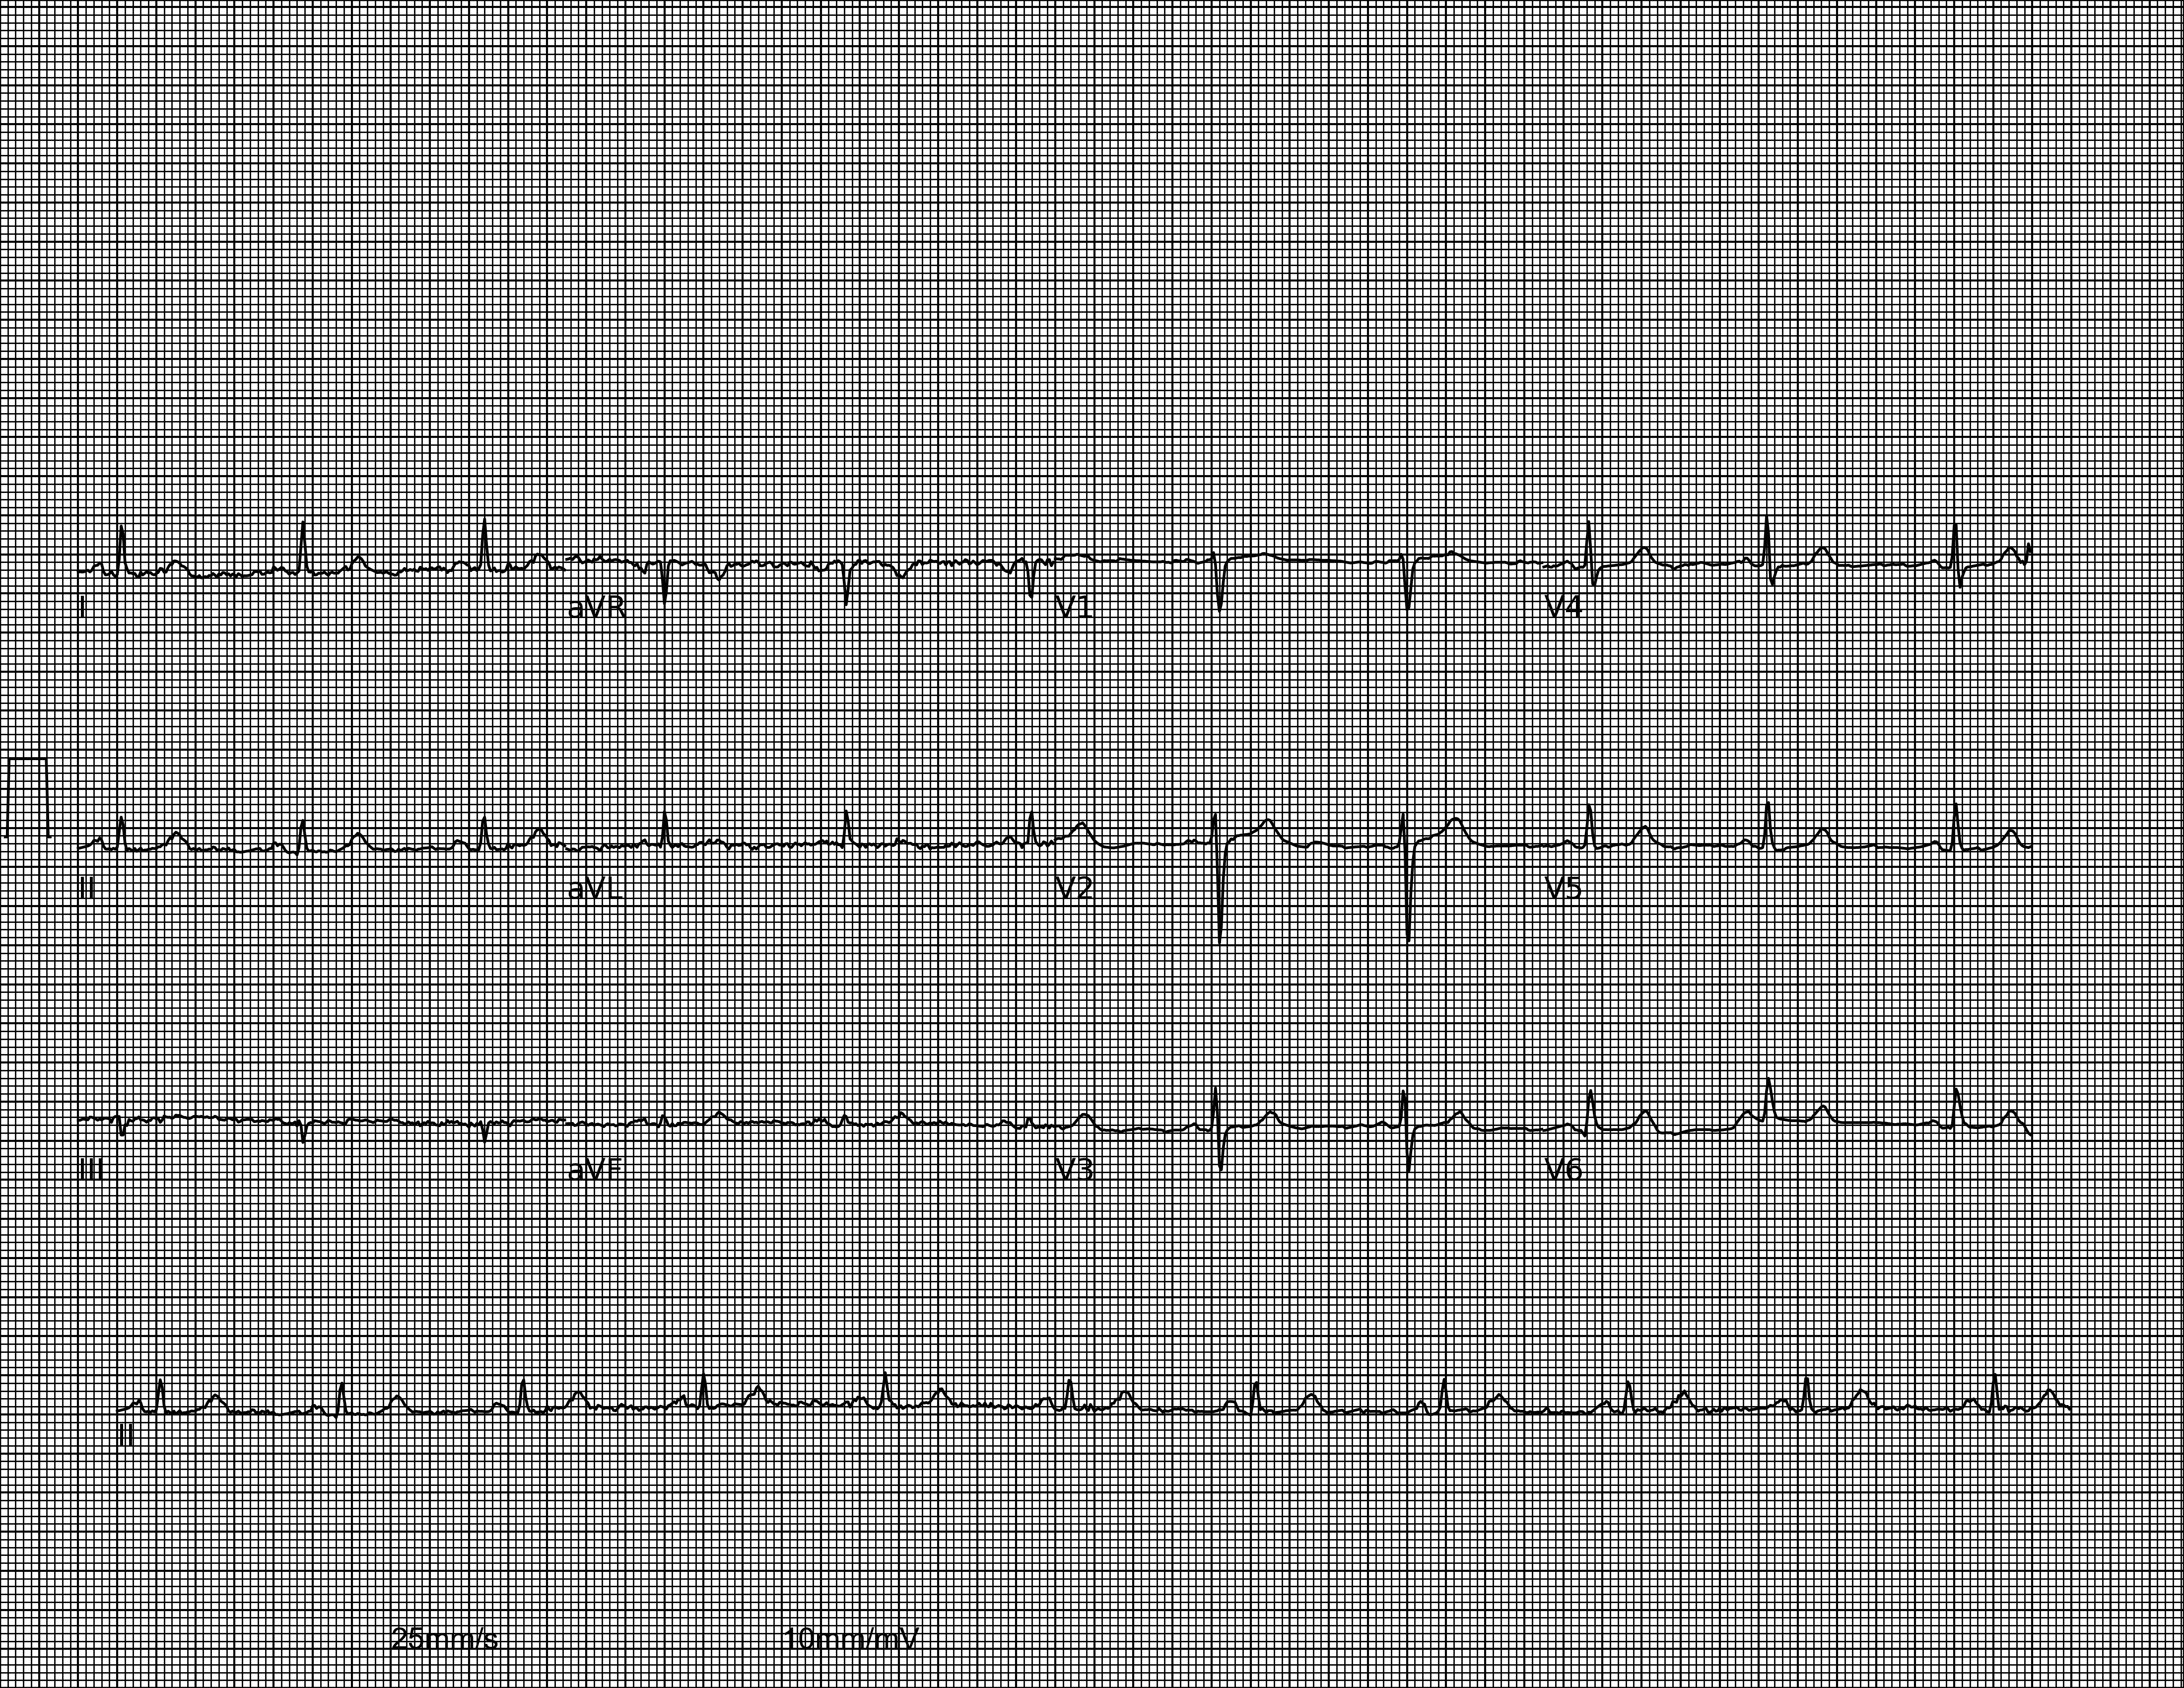
\includegraphics[width=\textwidth, trim={3.8in 2.8in 3.8in 2.8in}, clip]{images/sample_grid_normal.png}
        \caption{Griglia standard: linee minori continue.}
        \label{fig:grid_normal}
    \end{subfigure}
    \hfill
    \begin{subfigure}[t]{0.48\textwidth}
        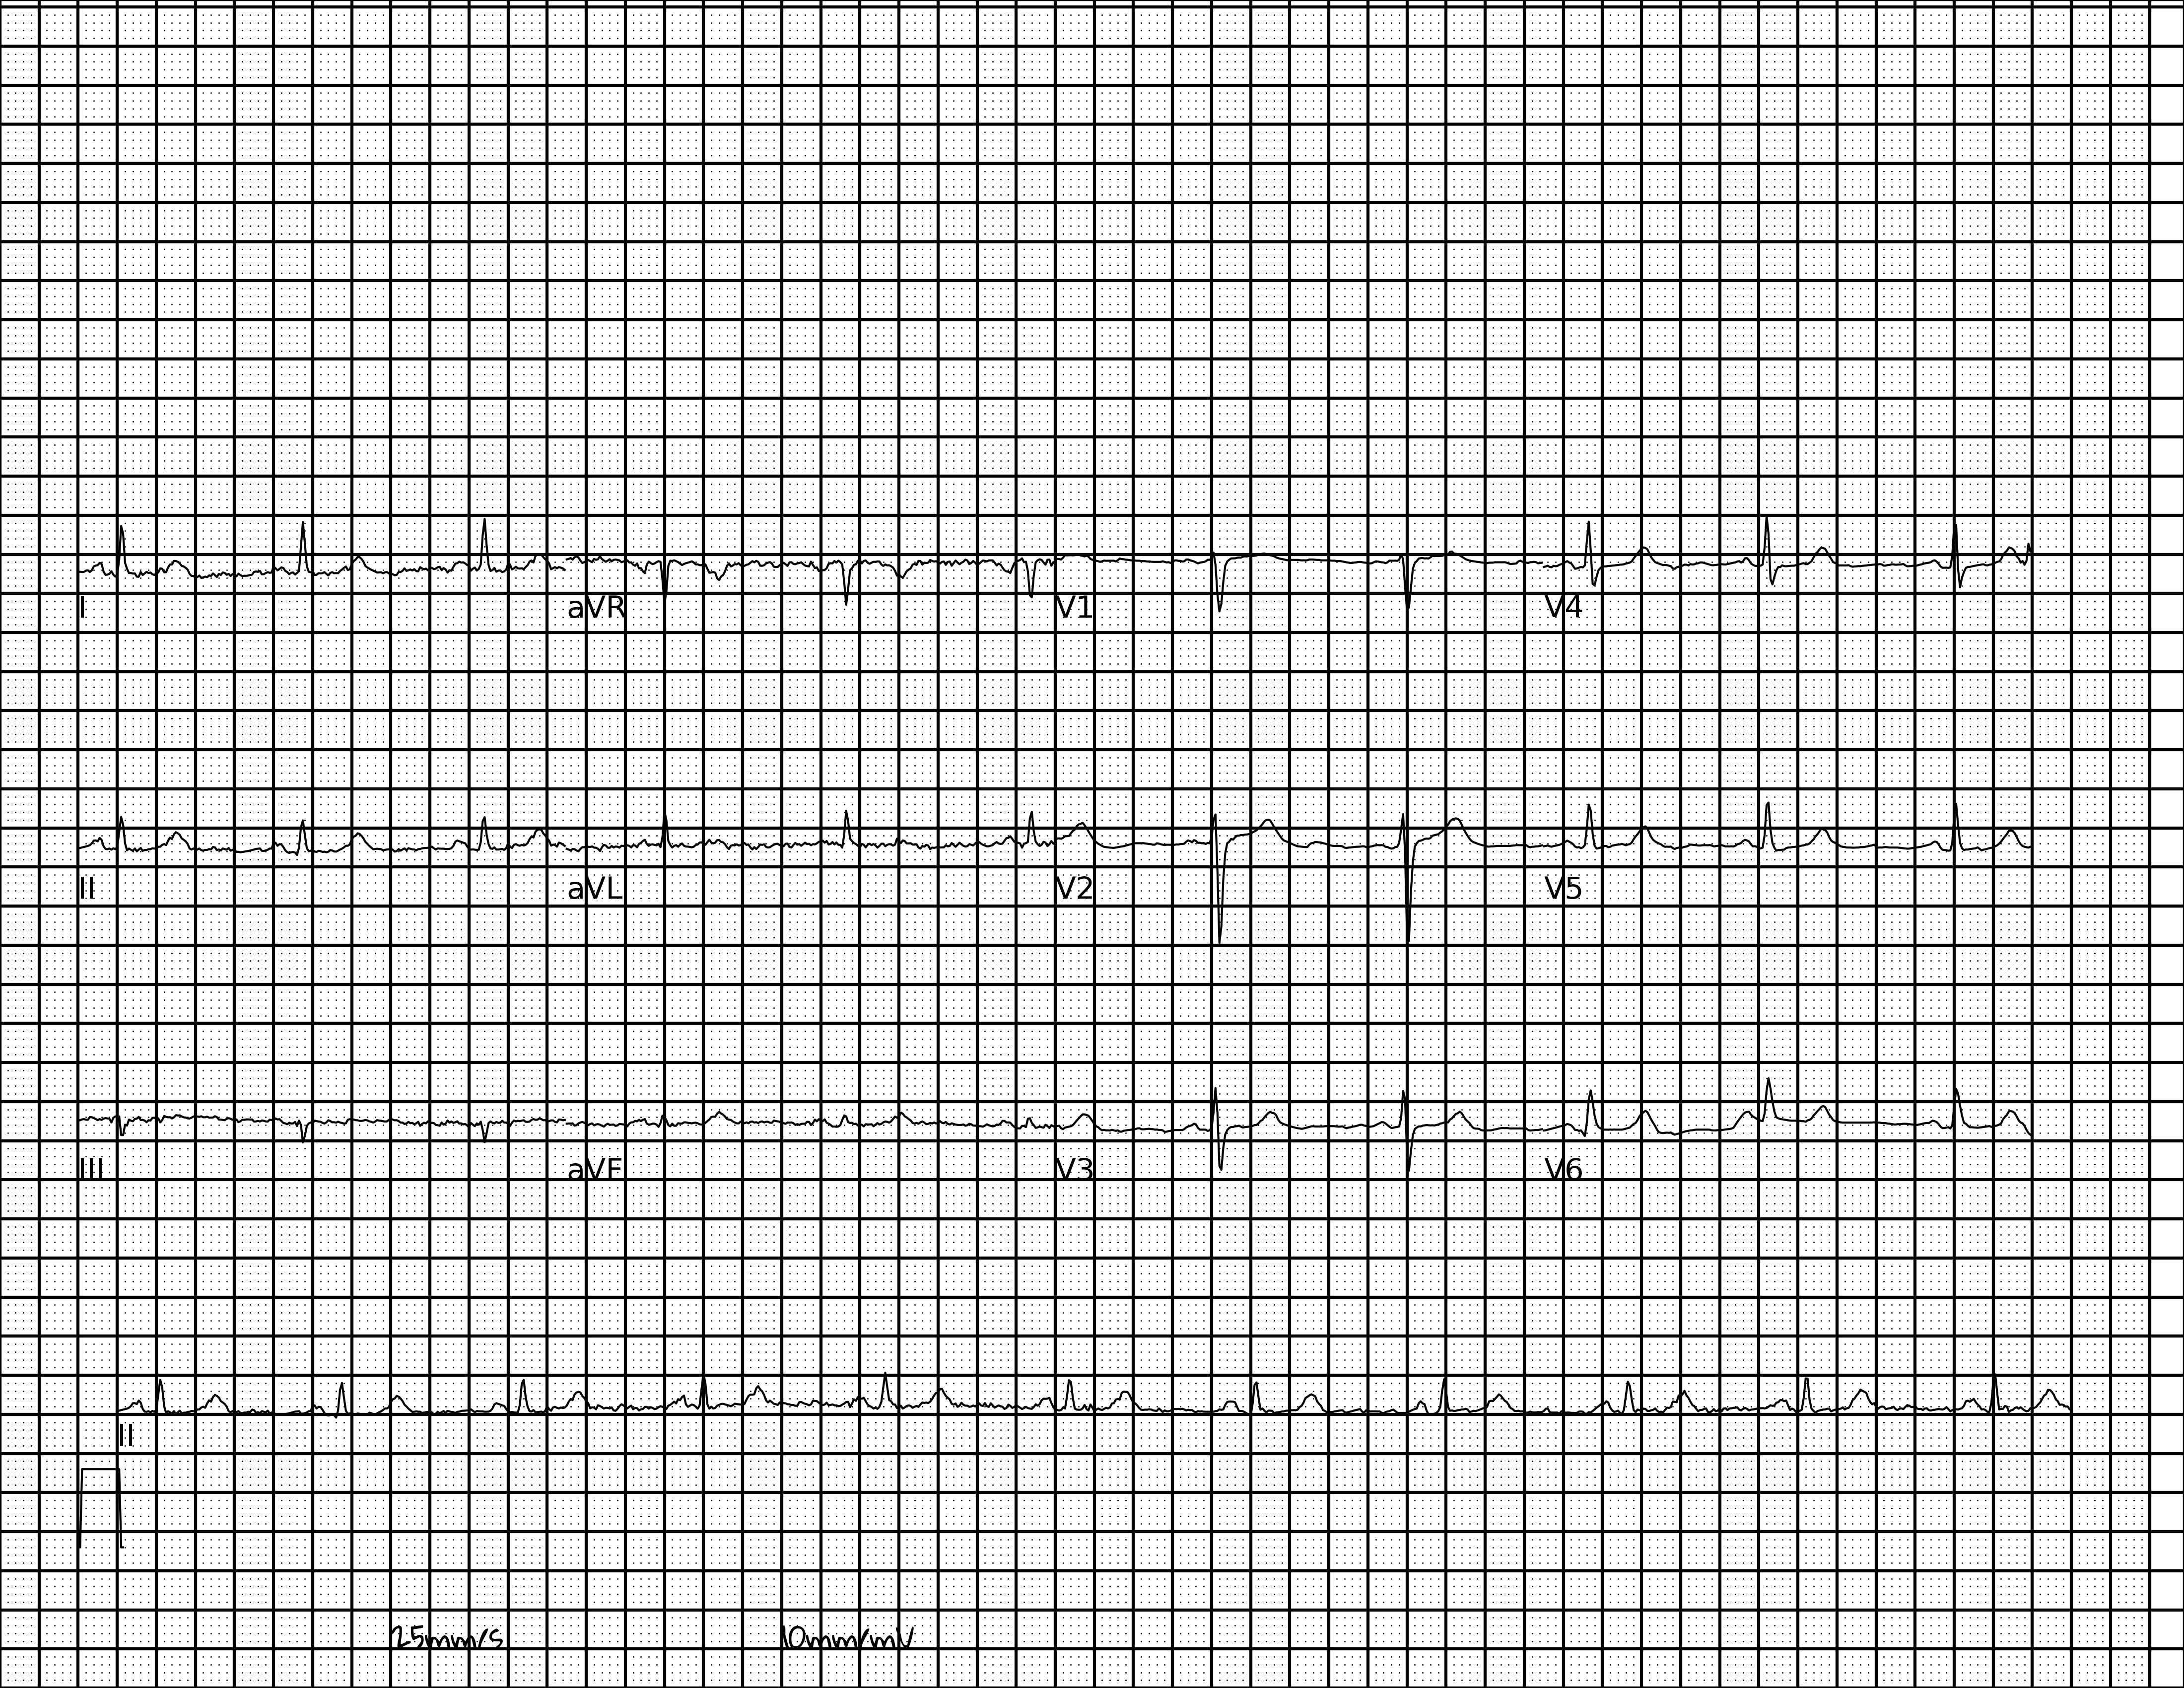
\includegraphics[width=\textwidth, trim={3.8in 2.8in 3.8in 2.8in}, clip]{images/sample_grid_dotted.png}
        \caption{Griglia dotted (\texttt{--prob\_dotted}): le linee minori sono sostituite da punti agli incroci.}
        \label{fig:grid_dotted_sub}
    \end{subfigure}
    \caption{Confronto tra griglia standard e griglia dotted (dettaglio centrale).}
    \label{fig:grid_dotted}
\end{figure}

\subsection{Impulso di Calibrazione}

L'impulso di calibrazione (o \textit{DC pulse}) è un'onda quadra di ampiezza 1 mV e durata 0.2 secondi posizionata a sinistra di ogni derivazione. Esso è presente negli ECG clinici come riferimento per la taratura dell'ampiezza. Il sistema supporta due modalità:

\begin{itemize}
    \item \textbf{Single:} un unico impulso posizionato sul lato sinistro dell'immagine, verticalmente centrato con un piccolo offset casuale sull'asse $y$ e un piccolo offset casuale sull'asse $x$, in modo che al più si sovrapponga con l'inizio di una delle derivazioni. È prevista la possibilità di clipping parziale, controllata da due parametri distinti: \texttt{--prob\_pulse\_clip} definisce la probabilità che l'impulso venga troncato, mentre \texttt{--pulse\_clip\_fraction} determina la frazione della durata rimossa. Il taglio avviene sempre dal lato sinistro: la porzione rimossa fuoriesce dal bordo dell'immagine, simulando realisticamente un'onda quadra acquisita parzialmente fuori campo.
    \item \textbf{Per lead:} un impulso per ogni derivazione, precedente al segnale.
\end{itemize}

\begin{figure}[H]
    \centering
    \begin{subfigure}[t]{0.48\textwidth}
        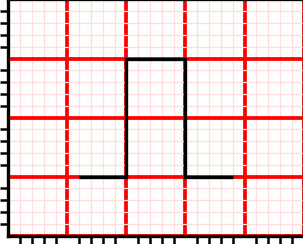
\includegraphics[width=\textwidth]{images/sample_pulse_full.png}
        \caption{Impulso di calibrazione completo: ampiezza 1~mV (2 quadretti), durata 0.2~s (1 quadretto).}
        \label{fig:pulse_full}
    \end{subfigure}
    \hfill
    \begin{subfigure}[t]{0.48\textwidth}
        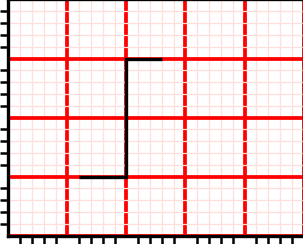
\includegraphics[width=\textwidth]{images/sample_pulse_clipped.png}
        \caption{Impulso troncato (\texttt{--prob\_pulse\_clip}): il taglio avviene sempre dal lato sinistro, con la porzione rimossa fuori dal bordo dell'immagine, simulando un'acquisizione parzialmente fuori campo.}
        \label{fig:pulse_clipped}
    \end{subfigure}
    \caption{Confronto tra impulso di calibrazione completo e clippato.}
    \label{fig:pulse_comparison}
\end{figure}

La probabilità che l'impulso sia presente in un'immagine è controllata da \texttt{--calibration\_pulse}. L'ampiezza e la durata dell'impulso sono parametrizzabili tramite \texttt{--dc\_pulse\_amplitude} e \texttt{--dc\_pulse\_duration}.

\subsection{Augmentation Geometrica in Fase di Rendering}

Un contributo apportato al sistema riguarda l'introduzione di perturbazioni geometriche direttamente nella fase di rendering, prima della rasterizzazione. Il parametro \texttt{--prob\_shift} definisce una probabilità unica applicata in modo indipendente a ciascun elemento visivo: ogni derivazione, ogni colonna, ogni impulso di calibrazione e ogni etichetta viene campionato separatamente, in modo che la traslazione possa essere applicata solo ad alcuni elementi e non ad altri nella stessa immagine. Gli spostamenti massimi ammissibili sono configurabili per ciascun tipo di elemento:

\begin{itemize}
    \item Traslazione verticale delle derivazioni: fino a \texttt{--max\_shift\_y} mV.
    \item Traslazione orizzontale delle colonne: fino a \texttt{--max\_shift\_col\_x} secondi.
    \item Traslazione orizzontale dell'impulso di calibrazione: fino a \texttt{--max\_shift\_pulse\_x}.
    \item Traslazione verticale dell'impulso di calibrazione: fino a \texttt{--max\_shift\_pulse\_y}.
    \item Traslazione dell'etichetta della derivazione: fino a \texttt{--max\_shift\_name}.
\end{itemize}

Questi spostamenti simulano le irregolarità di allineamento tipiche dei sistemi di stampa analogici e delle scansioni inclinate, aumentando la robustezza dei modelli addestrati su questo dato.

\subsection{Annotazioni e Bounding Box}

Per ogni derivazione, il sistema traccia la corrispondenza tra pixel dell'immagine e campioni del segnale, memorizzando le coordinate pixel di ogni punto plottato nel dizionario \texttt{json\_dict}. Sono inoltre disponibili le \textit{bounding box} che delimitano sia il tracciato del segnale (\texttt{--lead\_bbox}) che l'etichetta testuale (\texttt{--lead\_name\_bbox}). Ogni bounding box viene serializzata nel JSON come lista di quattro corner points nel formato \texttt{[[x1,y1],~[x2,y1],~[x2,y2],~[x1,y2]]}, dove i punti rappresentano i quattro vertici in senso orario a partire dall'angolo in alto a sinistra, in coordinate pixel \texttt{[x,~y]} con origine in alto a sinistra dell'immagine. A ciascun rettangolo viene applicato un margine fisso di \texttt{BBOX\_PADDING = 10} pixel per lato, definito in \texttt{ecg\_plot.py}, in modo da includere le variazioni di spessore del tratto attorno al profilo minimo. La scelta del formato a corner points, anziché del tradizionale asse-allineato \texttt{\{x1,~y1,~x2,~y2\}}, è motivata dalla pipeline di augmentation: dopo una rotazione, i quattro punti vengono trasformati individualmente dalla matrice di rotazione 2D e rappresentano il poligono realmente ruotato, senza perdita di informazione sull'orientamento (si veda la Sezione~\ref{sec:propagazione}). Queste annotazioni vengono serializzate in un file JSON per ogni immagine generata.

\subsection{Generazione dell'Immagine Pulita}

Il flag \texttt{--generate\_clean}, introdotto come nuova funzionalità, abilita la generazione contestuale di una versione pulita di ogni immagine: sfondo nero (tutti i pixel a 0) e tracciati bianchi (tutti i pixel a 1), senza griglia né artefatti. Le stesse trasformazioni geometriche applicate all'immagine principale, shift delle derivazioni, rotazione, vengono replicate sull'immagine pulita, garantendo la corrispondenza pixel-per-pixel tra le due. Questa immagine costituisce la \textit{ground truth} visiva per task di segmentazione semantica, consentendo ai modelli di apprendere la separazione tra segnale e disturbi.

\section{Output del Sistema e Configurazione JSON}\label{sec:output}

La pipeline di generazione opera interamente in memoria: il modulo di rendering restituisce l'immagine come oggetto Pillow in RAM, che viene passato in sequenza ai moduli di testo manoscritto, pieghe e augmentation senza mai scrivere file intermedi su disco. Questa scelta rappresenta un miglioramento rispetto alla repository originale, in cui ogni stadio della pipeline salvava l'immagine su disco per poi rileggerla allo stadio successivo, introducendo latenza di I/O non necessaria. Solo al termine dell'intera catena di elaborazione l'immagine finale (e l'eventuale ground truth pulita) viene serializzata nella directory di output. Questo approccio elimina la latenza di I/O degli stadi intermedi e riduce le operazioni di scrittura al minimo indispensabile, migliorando le prestazioni specialmente quando più processi generano immagini in parallelo e competono per l'accesso al disco.

Al termine della generazione di ogni immagine, il sistema produce i seguenti file:

\begin{itemize}
    \item \textbf{Immagine PNG sintetizzata:} il file immagine principale, con griglia, derivazioni, etichette e tutti gli artefatti richiesti. Se \texttt{--add\_qr\_code} è attivo, viene sovrapposto in alto a destra un codice QR che codifica il percorso relativo del file WFDB sorgente (campo \texttt{encoding} del record). Questo elemento permette di risalire univocamente alla registrazione originale a partire dalla sola immagine.
    \item \textbf{Immagine PNG pulita (opzionale):} la ground truth visiva, priva di griglia e disturbi.
    \item \textbf{File WFDB aggiornato:} una copia dei file \texttt{.hea} e \texttt{.dat} che riflette la segmentazione temporale applicata, con i campioni non visualizzati eventualmente mascherati con \texttt{NaN}.
    \item \textbf{File JSON di configurazione (opzionale):} serializza i parametri utilizzati per generare l'immagine (risoluzione, DPI della griglia, presenza del pulse di calibrazione, colori, flag di augmentation), nonché le coordinate delle bounding box e i pixel plottati per ogni derivazione. Il livello di dettaglio è controllato dal parametro \texttt{--store\_config} (livello 1: attributi di alto livello; livello 2: informazioni complete).
\end{itemize}

\section{Sistema di Configurazione}

La configurazione del sistema è stratificata su due livelli:

\begin{itemize}
    \item \textbf{File YAML (\texttt{config.yaml}):} contiene i parametri statici della griglia (durata della carta, passo della griglia, layout delle derivazioni per i diversi formati). Questi valori, originariamente fissi nel codice, sono stati estratti in questo file di configurazione come contributo originale al progetto, rendendo il sistema più facilmente adattabile a standard clinici diversi da quello di default.
    \item \textbf{Argomenti da riga di comando:} espongono oltre 50 parametri che controllano ogni aspetto della generazione, dal layout alla risoluzione, dai colori alle probabilità di applicazione di ciascun artefatto. Un principio trasversale a quasi tutti i parametri è la dualità \textit{deterministico/casuale}. Numerosi parametri numerici, come l'intensità del rumore, il livello di compressione JPEG o il grado di sfocatura, non rappresentano un valore fisso ma una soglia massima: il valore effettivo applicato a ciascuna immagine viene campionato casualmente nell'intervallo $[0, \text{valore}]$, introducendo variabilità automatica nel dataset senza richiedere configurazioni per ogni run. Questo comportamento stocastico è il default; per ottenere un valore deterministico e riproducibile è sufficiente affiancare il corrispondente flag \texttt{--deterministic\_*} (ad esempio \texttt{--deterministic\_noise}, \texttt{--deterministic\_blur}), che forza l'uso esatto del valore specificato invece di campionarlo. Alcuni parametri accettano inoltre il valore speciale \texttt{random} per delegare la scelta a un campionamento uniforme tra le opzioni disponibili: ad esempio, \texttt{--layout random} seleziona un formato tra quelli supportati in modo equiprobabile, e \texttt{--random\_grid\_color} genera ad ogni immagine una combinazione cromatica casuale per la griglia.
\end{itemize}

Questa architettura a due livelli separa nettamente i parametri strutturali del formato ECG (invarianti) dai parametri operativi della generazione (variabili per ogni run), consentendo di lanciare esperimenti con diverse configurazioni senza modificare il codice sorgente.

\vspace{4mm}
Nel prossimo capitolo verrà analizzata nel dettaglio la pipeline di artefatti, descrivendo i meccanismi con cui testo scritto a mano, pieghe e rugosità della carta e distorsioni fotometriche vengono iniettati sull'immagine sintetica per simulare le condizioni reali dei documenti clinici.
